\documentclass[11pt]{article}

\usepackage[margin=1in]{geometry}
\usepackage{graphicx}
\usepackage{booktabs}
\usepackage{amsmath}
\usepackage{amssymb}
\usepackage[numbers,sort&compress]{natbib}
\usepackage{caption}
\usepackage{subcaption}
\usepackage[hidelinks]{hyperref}
\usepackage[capitalise,nameinlink]{cleveref}
\crefname{figure}{Fig.}{Figs.}
\Crefname{figure}{Fig.}{Figs.}
\crefname{table}{Table}{Tables}
\crefname{section}{Section}{Sections}
\crefname{equation}{Eq.}{Eqs.}

\graphicspath{{figures/}}

% GENERATED by paper/sync_arxiv.py from ieee_bigdata/main.tex -- do not edit by hand.

\begin{document}

\title{Auditing SHAP Explanations Against Latent Failure Mechanisms in Predictive Maintenance}

\author{Koshik Debanath \\ \small Independent Researcher \\ \small \texttt{koshik.debanath@gmail.com}}
\date{}

\maketitle

\begin{abstract}
% X: what and why
Analysts use SHAP (SHapley Additive exPlanations) to explain predictive maintenance (PdM)
classifiers, but rarely test whether an explanation matches the physical cause of failure.
% Y: why hard
Such a test needs ground truth about why each failure happened, which PdM data rarely provides, and
we show that an obvious test for it certifies a model fitted to shuffled labels.
% Z: what we do
We use the AI4I~2020 dataset, whose failure label is the logical OR of separately recorded failure
mechanisms. We train a classifier on the combined label only, compute out-of-sample SHAP values by
cross-fitting, and test two statistics per mechanism against 1{,}000 models retrained on permuted
labels: the share of attribution on the mechanism's trigger features, and how much larger that
share is on the mechanism's rows than on other failures.
% 1: evidence
With Holm correction, the tuned XGBoost model (test F1 0.90) passes both tests for heat
dissipation, power, and overstrain failure in all five seeds (adjusted $p \le 0.02$), but not for tool wear
failure, which passes only when SHAP is computed on training rows. A graded shortcut experiment
shows that the audit flags a synthetic sensor once it carries about a third of the attribution on
the affected mechanism's rows, but not at 11\%, while test F1 stays between 0.85 and 0.92.
\end{abstract}

\noindent\textbf{Keywords:} 
explainable AI, SHAP, predictive maintenance, faithfulness evaluation, model randomization,
cyber-physical systems


\section{Introduction}
\label{sec:intro}

% X: explanations of PdM models are trusted without being tested against the true cause
Predictive maintenance (PdM) systems predict equipment failure from sensor readings of
cyber-physical systems, where a wrong reason for a correct alarm can send a technician to the wrong
component. Users typically explain these models with post-hoc attributions such as
SHAP~\cite{lundberg2017shap} and read the result as evidence that the model relies on sensible
inputs. The explanation itself is rarely tested against the actual cause of failure: a classifier
with high accuracy can still rely on a correlate of failure, and a plausible SHAP plot does not
reveal this~\cite{cummins2024survey}.

% Y: needs per-failure causes; naive tests are confounded
Testing an explanation against causes requires knowing, for each failure, which mechanism produced
it, and industrial datasets seldom record this. A second difficulty is statistical. Rows that belong
to a failure mechanism are extreme in that mechanism's features, and we find that a test which
ignores this effect passes a model fitted to shuffled labels (\cref{sec:robust}).

% Z: AI4I records mechanisms separately; we audit against them
The AI4I~2020 dataset~\cite{matzka2020explainable} records the mechanism of each failure. Its
target, \texttt{Machine failure}, is the logical OR of five flags: tool wear failure (TWF), heat
dissipation failure (HDF), power failure (PWF), overstrain failure (OSF), and random failure (RNF).
The first four follow published trigger rules on the sensor variables (\cref{tab:mechanisms}); RNF
does not. We train on the combined label only and keep the flags for an audit. For each mechanism,
we measure how much of the model's out-of-sample SHAP attribution falls on the features its trigger
rule uses, and whether that concentration is specific to its own rows, against models retrained on
permuted labels~\cite{adebayo2018sanity}.

% 1: hypotheses and outcomes
We test three hypotheses:
\begin{itemize}
  \item \textbf{H1:} for each physical mechanism, the model's attribution concentrates on the
    trigger features (1) more than permuted-label models do and (2) more on that mechanism's rows
    than on other failures;
  \item \textbf{H2:} the audit flags a model that relies on a shortcut sensor for the mechanism the
    shortcut imitates, while mechanisms that passed before keep passing;
  \item \textbf{H3:} a naive null, which compares random failure rows under the same model, does not
    separate a trained model from a permuted-label one.
\end{itemize}
H1 holds for HDF, PWF, and OSF but not for TWF (\cref{fig:overview}); H2 holds once the shortcut
carries about a third of the attribution; H3 holds.

\begin{figure}[htbp]
\centering
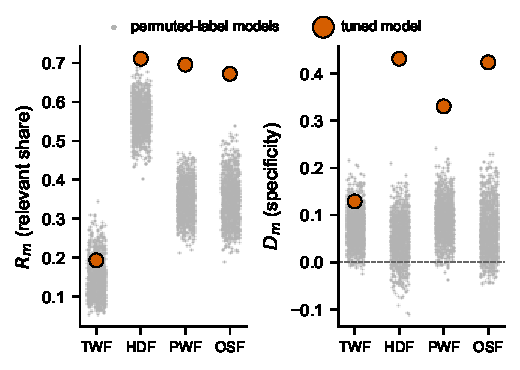
\includegraphics[width=0.55\textwidth]{audit_overview.pdf}
\caption{Out-of-sample audit statistics of the tuned model (orange) against 1{,}000
permuted-label models (gray). $R_m$ (\cref{eq:share}) is the relevant share and $D_m$
(\cref{eq:spec}) its excess on the mechanism's own rows. HDF, PWF, and OSF lie outside the null on
both; TWF does not on $R_m$.}
\label{fig:overview}
\end{figure}

% 2: contributions, separated from prior work
Our contributions are:
\begin{itemize}
  \item a per-mechanism SHAP audit with two statistics, out-of-sample attributions, a
    model-randomization null, and multiple-comparison correction (\cref{sec:method});
  \item evidence that a naive within-model null is confounded (\cref{sec:robust});
  \item a graded shortcut experiment that measures when the audit detects reliance on a spurious
    sensor (\cref{sec:sweep}), plus seed, single-mechanism, in-sample, and raw-feature analyses;
  \item an imbalance-aware benchmark of seven model families on AI4I~2020 with confidence
    intervals, and a code base that regenerates every number, table, and figure.
\end{itemize}
The resampling methods, models, explainer, and randomization idea are existing tools; the audit
statistics, the null analysis, and the controls are ours.

\section{Related Work}
\label{sec:related}

% XAI on AI4I: global reporting, no mechanism-level test; we compare predictive results
\textit{Explanations on AI4I~2020.} Matzka~\cite{matzka2020explainable} introduced the dataset with
local explanations of individual predictions, and Zhao et al.~\cite{milling2025shap} report global
SHAP importance for tree ensembles on it. Neither tests attributions against the mechanism flags or
defines a pass/fail criterion, so there is no audit to compare against. We compare predictive
performance instead: Tseng~\cite{physicsinformed2026} reports random forest positive-class F1 of
0.722, and Khemani and Qureshi~\cite{connectedvehicles2026} report LightGBM macro-F1 of
$0.814 \pm 0.012$ under 5-fold cross-validation with resampling inside the folds (\cref{tab:prior}).

% Ground-truth attribution benchmarks evaluate explainers; we evaluate models
\textit{Evaluating attributions against ground truth.} A line of work tests explainers on data where
the important features are known by construction: XAI-Bench~\cite{liu2021synthetic} and
OpenXAI~\cite{agarwal2022openxai} generate synthetic tabular data, BAM~\cite{yang2019bam} and Zhou
et al.~\cite{zhou2022attribute} modify images or text so that a known feature drives the label, and
CLEVR-XAI~\cite{arras2022clevr} provides ground-truth masks for visual questions.
ROAR~\cite{hooker2019roar} avoids ground truth by retraining after removing the features an
explainer ranks highest. These methods ask whether an explainer reports what the model uses. We ask
the complementary question: given TreeSHAP, whose values are exact for tree ensembles, does the
model use what the data-generating mechanism uses? The benchmarks above control the data-generating
process, which AI4I~2020 does not expose beyond its trigger rules, so we do not run them as
baselines. Chen et al.~\cite{chen2020true} distinguish attributions that are ``true to the model''
from ones ``true to the data''; our audit targets the second property at the level of mechanism
subgroups.

% Randomization tests: adopted, applied to the model
\textit{Randomization tests.} Adebayo et al.~\cite{adebayo2018sanity} show that some saliency
methods give nearly the same explanation for a trained model and a randomized one. We apply the same
logic to the model rather than the explainer: permuted-label models define what attribution looks
like without any relation to the failure mechanisms.

% Causal PdM: different goal
\textit{Causal PdM.} Dhande et al.~\cite{causalbenchmark2026} fit causal structural models on a CNC
failure dataset of similar size to optimize maintenance cost. They replace the correlational model;
we keep it and test its explanation.

\section{Background and Problem Setting}
\label{sec:background}

% SHAP basics
\textit{SHAP.} For a model $f$ and input $x$ with $d$ features, SHAP assigns each feature $j$ an
attribution $\phi_j(x)$, its Shapley value with respect to the model output, such that
$f(x) = \phi_0 + \sum_{j=1}^{d} \phi_j(x)$, where $\phi_0$ is the expected
output~\cite{lundberg2017shap}. TreeSHAP computes these values exactly for tree ensembles. We use
$|\phi_j(x)|$ as the magnitude of feature $j$'s contribution to the prediction for $x$.

% Problem setting and notation
\textit{Problem setting.} We observe rows $(x_i, y_i, z_i)$, where $x_i$ is the sensor vector,
$y_i \in \{0, 1\}$ the failure label, and $z_i \in \{0, 1\}^M$ holds $M$ mechanism flags. We train
$f$ on $(x_i, y_i)$ only. For each mechanism $m$, domain rules give a set $E_m$ of features the
mechanism's trigger depends on. With $S_m = \{i : z_{i,m} = 1\}$ and $F = \{i : y_i = 1\}$, the
audit asks whether attributions on $S_m$ concentrate on $E_m$, and more so than on $F \setminus S_m$.
Two assumptions are unusual: $E_m$ must be known, and the flags must exist for some failures even
though the model never sees them.

\section{Audit Method}
\label{sec:method}

% Statistics
For a set of rows $S$ and mechanism $m$, let
$I_{m,j}(S) = |S|^{-1} \sum_{i \in S} |\phi_j(x_i)|$ and define the share of attribution on the
trigger features,
\begin{equation}
  r_m(S) = \sum_{j \in E_m} I_{m,j}(S) \Big/ \sum_{j=1}^{d} I_{m,j}(S).
\end{equation}
The audit uses two statistics, the \textit{relevant share} and the \textit{specificity},
\begin{align}
  R_m &= r_m(S_m), \label{eq:share} \\
  D_m &= r_m(S_m) - r_m(F \setminus S_m). \label{eq:spec}
\end{align}
$R_m$ is large when attribution on the mechanism's rows falls on its trigger features; $D_m$ is
large when this concentration is specific to those rows rather than common to all failures.

% Out-of-sample attributions
\textit{Out-of-sample attributions.} Attributions on training rows reflect what the model fitted,
not what it generalizes. We therefore cross-fit: we split the data into five stratified folds, train
the full pipeline on four, and compute SHAP values for the held-out fold, so that every audited row
is explained by a model that never saw it.

% Naive null and its confound
\textit{Naive null.} An obvious test compares $R_m$ with the same statistic on random, equally sized
subsets of $F$ under the same model. It passes a model fitted to shuffled labels
(\cref{sec:robust}). A likely reason is that rows in $S_m$ are extreme in the features of $E_m$,
because the trigger rule selects them by those features, and $|\phi_j|$ tends to be larger at
atypical feature values whatever the model has fitted.

% Model-randomization null, p-values, correction
\textit{Model-randomization null.} We rerun the full procedure -- features, resampling,
hyperparameters, and cross-fitting -- $K$ times on permuted labels and compute both statistics for
each run. For $T \in \{R_m, D_m\}$ with null values $T^{(k)}$,
\begin{equation}
  p = \frac{1 + \#\{k : T^{(k)} \ge T\}}{K + 1},
\end{equation}
and we adjust the four physical mechanisms for multiple comparisons with Holm's method, separately
for each statistic. A mechanism passes a test if its adjusted $p$ is below 0.05.

% RNF
\textit{Random failures.} RNF has no trigger features. We report the share of its single largest
feature and whether it is more concentrated than under the null, as a descriptive check rather
than a pass/fail test.

\section{Experimental Setup}
\label{sec:setup}

% Dataset and label inconsistencies
\textit{Dataset.} AI4I~2020 has 10{,}000 rows: a quality variant \texttt{Type} $\in \{L, M, H\}$,
five process variables (air and process temperature, rotational speed, torque, tool wear), the
failure label, and the five mechanism flags. 339 rows (3.39\%) are failures. The labels depart from
the stated OR rule: 24 rows carry several mechanism flags, 9 failures carry none, and 18 of the 19
RNF rows have \texttt{Machine failure}~$= 0$, which is why we treat RNF descriptively. We audit all
flagged rows and, separately, rows with exactly one flag.

\begin{table}[htbp]
\centering
\caption{Failure mechanisms in AI4I~2020~\cite{matzka2020explainable} and their trigger features
$E_m$; counts as released. The TWF failure point is random within the window.}
\label{tab:mechanisms}
\footnotesize
\setlength{\tabcolsep}{3pt}
\begin{tabular}{@{}lp{3.4cm}p{2.9cm}r@{}}
\toprule
Mech. & Trigger & $E_m$ & $n$ \\
\midrule
TWF & tool wear at a random point in 200--240\,min & tool wear & 46 \\
HDF & (process $-$ air temp.) $< 8.6$\,K and speed $< 1380$\,rpm & both temps., their difference,
  speed & 115 \\
PWF & torque $\times$ speed (rad/s) outside [3500, 9000]\,W & torque, speed, power & 95 \\
OSF & tool wear $\times$ torque above 11{,}000/12{,}000/13{,}000\,min$\cdot$Nm for L/M/H & tool
  wear, torque, overstrain, its ratio & 98 \\
RNF & 0.1\% chance, independent of the process & -- & 19 \\
\bottomrule
\end{tabular}
\end{table}

% Features
\textit{Features.} We derive four features from the trigger rules without using the flags:
\textit{power} (torque $\times$ speed), \textit{temperature difference} (process $-$ air),
\textit{overstrain} (tool wear $\times$ torque), and \textit{overstrain ratio} (overstrain over the
type-specific limit). The mechanism flags are components of the label, so we exclude them from the
features.

% Training
\textit{Training.} We split the data 70/20/10 into training, validation, and test sets, stratified by
label, and fit scaling and one-hot encoding on the training set. We compare three oversamplers --
SMOTE~\cite{chawla2002smote}, Borderline-SMOTE~\cite{han2005borderline}, and
ADASYN~\cite{he2008adasyn} -- by the validation F1 of a default XGBoost~\cite{chen2016xgboost} model
and use the best, Borderline-SMOTE (\cref{tab:resamplers}). We train seven model families
(\cref{tab:config}; the tuned XGBoost is the eighth row, not a separate family).

\begin{table}[htbp]
\centering
\caption{Model settings. Unlisted hyperparameters are library defaults (scikit-learn 1.9.1,
XGBoost 3.4.1, PyTorch 2.14.0); random seed 42.}
\label{tab:config}
\footnotesize
\begin{tabular}{@{}lp{5.6cm}@{}}
\toprule
Model & Settings \\
\midrule
Logistic regression & max.\ 1000 iterations \\
SVM & radial basis function (RBF) kernel, probability outputs \\
$k$-NN & $k = 7$ \\
Decision tree & max.\ depth 10 \\
Random forest & 300 trees, max.\ depth 12 \\
XGBoost & 300 trees, max.\ depth 6, learning rate 0.1 \\
XGBoost (tuned) & 200 trees, max.\ depth 8, learning rate 0.2, subsample 0.8, column sample 1.0, min.\ child weight 1, $\gamma = 0$ \\
MLP & 64 and 32 hidden units, ReLU, batch norm, dropout 0.3/0.2; Adam (learning rate $10^{-3}$, weight decay $10^{-5}$), binary cross-entropy, batch 64, 40 epochs \\
\bottomrule
\end{tabular}

\end{table}

% Selection, tuning, uncertainty
\textit{Selection and tuning.} We select on the validation set only: XGBoost has the highest
validation F1, so we tune it with a 40-iteration randomized search under 5-fold stratified
cross-validation, scored on F1, over depth 3--8, 200--600 trees, learning rate 0.01--0.2,
subsample and column sample 0.6--1.0, minimum child weight 1--5, and $\gamma$ 0--0.3. We set the
decision threshold to maximize F1 on the validation precision-recall (PR) curve. Confidence intervals
(CIs) are exact binomial (Clopper--Pearson) for precision and recall and a 5{,}000-sample stratified
bootstrap otherwise. We also run 5-fold stratified cross-validation of the whole pipeline at the
default threshold of 0.5.

% Audit configuration and cost
\textit{Audit.} The primary audit cross-fits the tuned pipeline with seed 42 and $K = 1{,}000$
permuted-label runs, so the smallest attainable $p$ before correction is 0.001. We repeat it with
seeds 1--4 ($K = 200$), with raw features only (without the four derived features, to test whether
they make the audit circular), and with SHAP computed on a single model's training rows
(\textit{in-sample}). Each run costs $5(K+1)$ model fits; the runs are independent, and the primary
audit takes 11 minutes on eight CPU cores.

% Controls
\textit{Controls.} A model trained on permuted labels is exchangeable with the null runs, so its
$p$-values are uniform by construction; we use it only as a sanity check of the code and as the
case that the naive null must fail. For H2, we add a synthetic ``sensor''
$s = z_{\mathrm{HDF}} + \mathcal{N}(0, \sigma^2)$ with no physical role and vary $\sigma$ from 2 to
0.1. For each $\sigma$ we report the sensor's share of attribution on HDF rows, test F1, and the
audit verdicts ($K = 100$). The sensor is not in $E_{\mathrm{HDF}}$, so a model that relies on it
should fail the HDF audit.

\section{Results and Discussion}
\label{sec:results}

\begin{figure}[htbp]
\centering
\begin{minipage}[b]{0.49\textwidth}
\centering
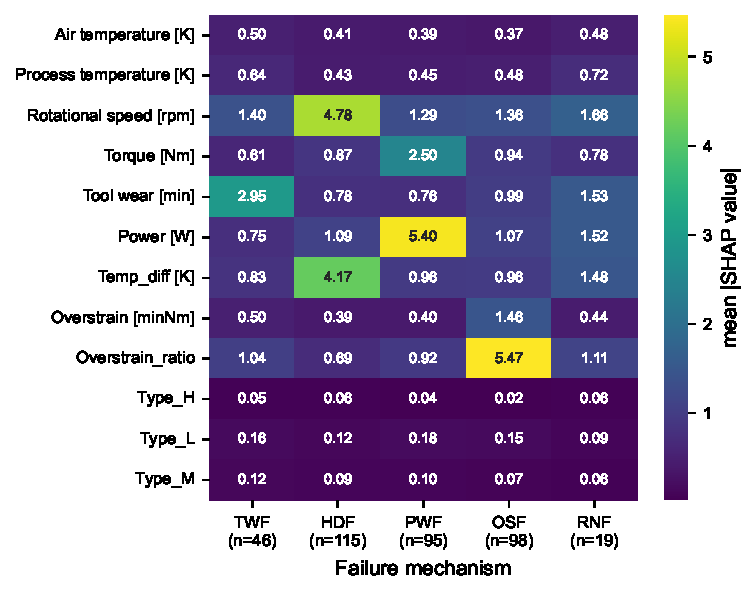
\includegraphics[width=0.93\linewidth]{shap_crosscheck_heatmap.pdf}\\
\small (a) Mean out-of-sample $|\phi_j|$ on the rows of each mechanism
\end{minipage}\hfill
\begin{minipage}[b]{0.47\textwidth}
\centering
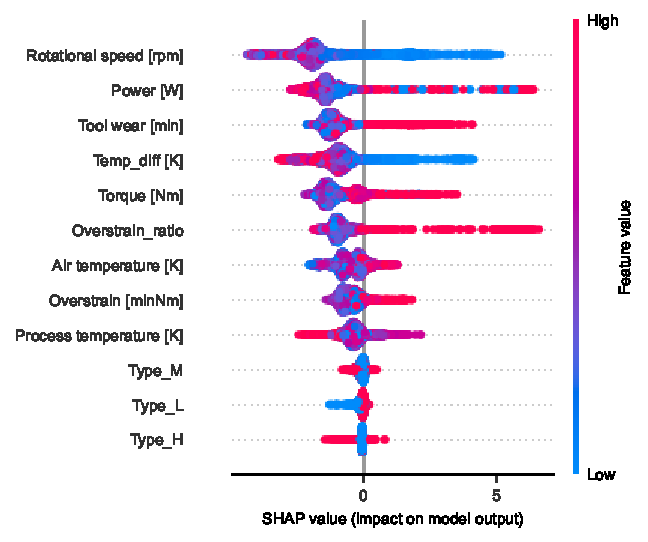
\includegraphics[width=0.93\linewidth]{shap_summary.pdf}\\
\small (b) Global SHAP summary on all rows
\end{minipage}
\caption{SHAP attributions of the tuned model. The audit tests the per-mechanism view (a); the global
view (b) ranks features overall but does not separate the mechanisms.}
\label{fig:shap}
\end{figure}

\begin{table}[htbp]
\centering
\caption{Primary audit (cross-fitted, seed 42, $K = 1{,}000$). Null: mean over permuted-label runs.
$p$: Holm-adjusted over the four physical mechanisms; $^{\times}$ marks $p \ge 0.05$. For RNF the
statistic is the largest feature's share and $p$ tests for more concentration than the null.}
\label{tab:audit}
\footnotesize
\begin{tabular}{@{}lrlrrrrrr@{}}
\toprule
& $n$ & Top feature & $R_m$ & Null & $p$ & $D_m$ & Null & $p$ \\
\midrule
TWF & 46 & speed & 0.203 & 0.147 & 0.096$^{\times}$ & 0.126 & 0.060 & 0.039 \\
HDF & 115 & speed & 0.726 & 0.553 & 0.004 & 0.413 & 0.041 & 0.004 \\
PWF & 95 & power & 0.671 & 0.336 & 0.004 & 0.288 & 0.065 & 0.004 \\
OSF & 98 & overstrain ratio & 0.625 & 0.339 & 0.004 & 0.388 & 0.054 & 0.004 \\
RNF & 19 & speed & 0.200 & 0.221 & 0.841 & -- & -- & -- \\
\bottomrule
\end{tabular}

\end{table}

\begin{table}[htbp]
\centering
\caption{Holm-adjusted audit $p$-values for $R_m$ and $D_m$ across analysis variants;
$^{\times}$ marks $p \ge 0.05$. The smallest attainable adjusted $p$ is $4/(K+1)$. The permuted-label
model is exchangeable with its null and serves only as a sanity check; the last row applies the
naive null of \cref{sec:method} to that model.}
\label{tab:robust}
\footnotesize
\begin{tabular}{@{}lrrrrrrrrr@{}}
\toprule
& & \multicolumn{2}{c}{TWF} & \multicolumn{2}{c}{HDF} & \multicolumn{2}{c}{PWF} & \multicolumn{2}{c}{OSF} \\
\cmidrule(lr){3-4}\cmidrule(lr){5-6}\cmidrule(lr){7-8}\cmidrule(lr){9-10}
Variant & $K$ & $R$ & $D$ & $R$ & $D$ & $R$ & $D$ & $R$ & $D$ \\
\midrule
Primary, seed 42 & 1000 & 0.201$^{\times}$ & 0.077$^{\times}$ & 0.004 & 0.004 & 0.004 & 0.004 & 0.004 & 0.004 \\
\quad single-mechanism rows & 1000 & 0.187$^{\times}$ & 0.076$^{\times}$ & 0.004 & 0.004 & 0.004 & 0.004 & 0.004 & 0.004 \\
Seed 1 & 200 & 0.199$^{\times}$ & 0.119$^{\times}$ & 0.020 & 0.020 & 0.020 & 0.020 & 0.020 & 0.020 \\
Seed 2 & 200 & 0.149$^{\times}$ & 0.065$^{\times}$ & 0.020 & 0.020 & 0.020 & 0.020 & 0.020 & 0.020 \\
Seed 3 & 200 & 0.174$^{\times}$ & 0.095$^{\times}$ & 0.020 & 0.020 & 0.020 & 0.020 & 0.020 & 0.020 \\
Seed 4 & 200 & 0.269$^{\times}$ & 0.129$^{\times}$ & 0.020 & 0.020 & 0.020 & 0.020 & 0.020 & 0.020 \\
Raw features only & 1000 & 0.345$^{\times}$ & 0.616$^{\times}$ & 0.190$^{\times}$ & 0.004 & 0.004 & 0.004 & 0.004 & 0.048 \\
In-sample SHAP & 1000 & 0.004 & 0.004 & 0.004 & 0.004 & 0.004 & 0.004 & 0.004 & 0.004 \\
Interventional TreeSHAP & 200 & 0.020 & 0.020 & 0.020 & 0.020 & 0.020 & 0.020 & 0.020 & 0.020 \\
Random forest & 200 & 0.617$^{\times}$ & 0.398$^{\times}$ & 0.020 & 0.020 & 0.020 & 0.020 & 0.040 & 0.020 \\
Permuted labels (sanity) & 200 & 1.000$^{\times}$ & 0.731$^{\times}$ & 0.199$^{\times}$ & 0.557$^{\times}$ & 1.000$^{\times}$ & 0.731$^{\times}$ & 1.000$^{\times}$ & 0.731$^{\times}$ \\
\midrule
Naive null, tuned model & -- & 0.002 & -- & 0.002 & -- & 0.002 & -- & 0.002 & -- \\
Naive null, permuted labels & -- & 0.002 & -- & 0.002 & -- & 0.002 & -- & 0.002 & -- \\
\bottomrule
\end{tabular}

\end{table}

\subsection{Predictive performance}
\label{sec:perf}

% Results table, uncertainty
\Cref{tab:models} lists test metrics. Tree ensembles outperform the linear and instance-based
models. Tuning raises F1 from 0.87 to 0.90, mainly through precision. The test set holds 34 failures,
so the uncertainty is large: the tuned model flags 28 rows, all true failures, which gives precision
1.00 (95\% CI 0.88--1.00) and recall 0.82 (0.65--0.93). Its scores are calibrated (Brier score
0.0095 against 0.033 for a constant prediction at the base rate; expected calibration error 0.007).
Five-fold cross-validation of the full pipeline gives positive-class F1 $0.823 \pm 0.016$ and
macro-F1 $0.908 \pm 0.009$, against the $0.814 \pm 0.012$ macro-F1 that Khemani and
Qureshi~\cite{connectedvehicles2026} report for LightGBM under a comparable protocol
(\cref{tab:prior}). \Cref{fig:pr,fig:cm} show PR curves and the confusion matrix.

\begin{table}[htbp]
\centering
\caption{Positive-class test metrics, sorted by F1; bootstrap 95\% CI for F1.}
\label{tab:models}
\footnotesize
\setlength{\tabcolsep}{4pt}
\begin{tabular}{@{}lrrlr@{}}
\toprule
Model & Prec. & Rec. & F1 (95\% CI) & ROC-AUC \\
\midrule
XGBoost (tuned) & \textbf{1.00} & 0.82 & \textbf{0.90} (0.81--0.97) & 0.984 \\
XGBoost & 0.86 & 0.88 & 0.87 (0.78--0.94) & 0.988 \\
Random forest & 0.79 & 0.88 & 0.83 (0.74--0.92) & \textbf{0.989} \\
MLP & 0.65 & \textbf{0.91} & 0.76 (0.67--0.84) & 0.988 \\
Decision tree & 0.68 & 0.82 & 0.75 (0.64--0.84) & 0.927 \\
SVM & 0.42 & 0.88 & 0.57 (0.48--0.65) & 0.976 \\
k-NN & 0.43 & 0.79 & 0.56 (0.46--0.65) & 0.877 \\
Logistic regression & 0.24 & 0.85 & 0.37 (0.31--0.43) & 0.943 \\
\bottomrule
\end{tabular}

\end{table}

\begin{table}[htbp]
\centering
\caption{Comparison with prior results on AI4I~2020.}
\label{tab:prior}
\footnotesize
\begin{tabular}{@{}llr@{}}
\toprule
Study and protocol & Metric & Value \\
\midrule
Random forest, single split~\cite{physicsinformed2026} & pos.-class F1 & 0.722 \\
LightGBM, 5-fold CV~\cite{connectedvehicles2026} & macro-F1 & $0.814 \pm 0.012$ \\
Ours, single split & pos.-class F1 & 0.90 \\
Ours, 5-fold CV & pos.-class F1 & $0.823 \pm 0.016$ \\
Ours, 5-fold CV & macro-F1 & $0.908 \pm 0.009$ \\
\bottomrule
\end{tabular}

\end{table}

\begin{figure}[htbp]
\centering
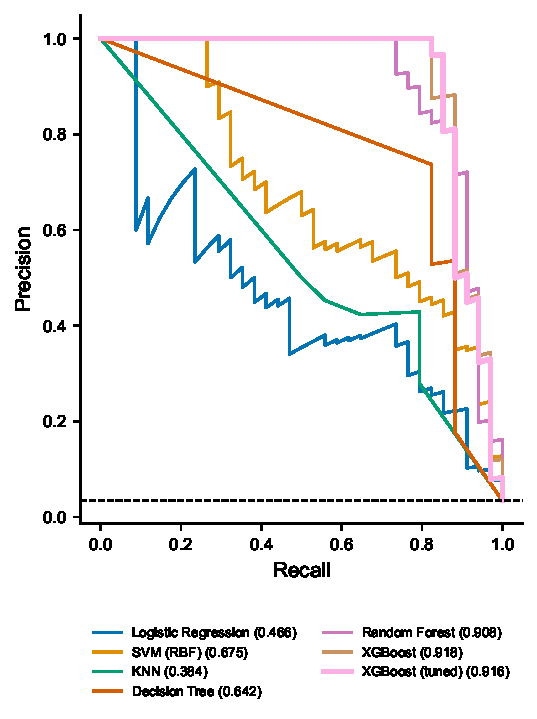
\includegraphics[width=0.40\textwidth]{pr_curves.pdf}
\caption{Test PR curves (average precision in parentheses); the dashed line is the 3.4\% failure
rate.}
\label{fig:pr}
\end{figure}

\begin{figure}[htbp]
\centering
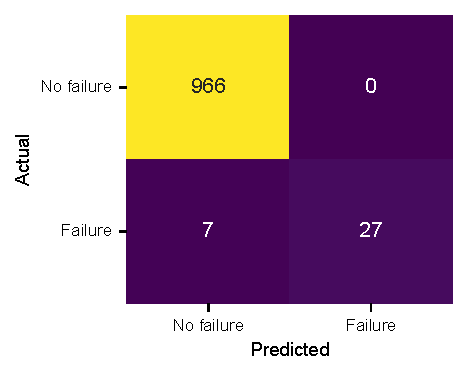
\includegraphics[width=0.30\textwidth]{confusion_matrix_best.pdf}
\caption{Confusion matrix of the tuned model on the test set.}
\label{fig:cm}
\end{figure}

\subsection{Audit of the tuned model (H1)}
\label{sec:audit-results}

% H1 supported for HDF, PWF, OSF
For HDF, PWF, and OSF the tuned model passes both tests (\cref{tab:audit}, \cref{fig:overview}). On
each mechanism's held-out rows, the share of attribution on its trigger features exceeds that of
every permuted-label run, and it exceeds the share on other failures by 0.29 to 0.41, against
null means below 0.07. The highest-attribution feature is a trigger feature in each case.
\Cref{fig:shap}a shows the attribution matrix.

% H1 not supported for TWF
TWF fails the relevant-share test ($p = 0.096$). Its specificity passes ($p = 0.039$), but its
highest-attribution feature out-of-sample is rotational speed, not tool wear. The TWF trigger fires
at a random point within a tool-wear window, so tool wear only partly determines it, and the 46 TWF
rows give little to generalize from.

\subsection{Robustness (H1, H3)}
\label{sec:robust}

% Seeds, single rows
\Cref{tab:robust} repeats the audit. The HDF, PWF, and OSF verdicts hold in all five seeds and on
single-mechanism rows. TWF fails the relevant-share test in every seed, and its specificity passes in
three of five, so we do not count TWF as supported.

% In-sample optimism
With SHAP computed on training rows, all four mechanisms pass, including TWF ($p = 0.008$). The
difference from the cross-fitted result shows that in-sample attributions can overstate how well a
model's explanation matches a mechanism.

% Raw features: circularity partly addressed
Without the derived features, PWF passes both tests, HDF passes only on specificity, OSF only on the
relevant share, and TWF on neither. The derived features therefore contribute to the audit
outcomes, so the circularity concern is only partly resolved; mechanisms defined by a difference or
product of inputs are harder to audit when the model must approximate that quantity with splits.

% H3 and sanity
The permuted-label model fails every test under the model-randomization null, as it must. The naive
null passes the same model on all four mechanisms (Holm-adjusted $p = 0.002$), which supports H3.

\subsection{Shortcut sweep (H2)}
\label{sec:sweep}

\begin{table}[htbp]
\centering
\caption{Shortcut sweep ($K = 100$): test F1, the sensor's share of attribution on HDF rows,
$R_{\mathrm{HDF}}$, and Holm-adjusted HDF $p$-values; $^{\times}$ marks $p \ge 0.05$.}
\label{tab:sweep}
\footnotesize
\setlength{\tabcolsep}{3pt}
\begin{tabular}{@{}rrrrrrl@{}}
\toprule
$\sigma$ & F1 & Sensor share & $R_{\mathrm{HDF}}$ & $p_R$ & $p_D$ & PWF, OSF \\
\midrule
2.0 & 0.90 & 0.025 & 0.705 & 0.008 & 0.008 & pass \\
1.0 & 0.89 & 0.023 & 0.695 & 0.008 & 0.008 & pass \\
0.67 & 0.88 & 0.033 & 0.678 & 0.008 & 0.008 & pass \\
0.5 & 0.85 & 0.051 & 0.656 & 0.008 & 0.008 & pass \\
0.4 & 0.89 & 0.080 & 0.621 & 0.008 & 0.008 & pass \\
0.35 & 0.92 & 0.126 & 0.574 & 0.044 & 0.008 & pass \\
0.3 & 0.90 & 0.209 & 0.475 & 0.365$^{\times}$ & 0.008 & pass \\
0.25 & 0.87 & 0.350 & 0.308 & 0.996$^{\times}$ & 0.012 & pass \\
0.2 & 0.90 & 0.425 & 0.222 & 1.000$^{\times}$ & 0.084$^{\times}$ & pass \\
0.15 & 0.84 & 0.456 & 0.185 & 1.000$^{\times}$ & 0.168$^{\times}$ & pass \\
0.1 & 0.87 & 0.405 & 0.218 & 1.000$^{\times}$ & 0.068$^{\times}$ & pass \\
\bottomrule
\end{tabular}

\end{table}

\begin{figure}[htbp]
\centering
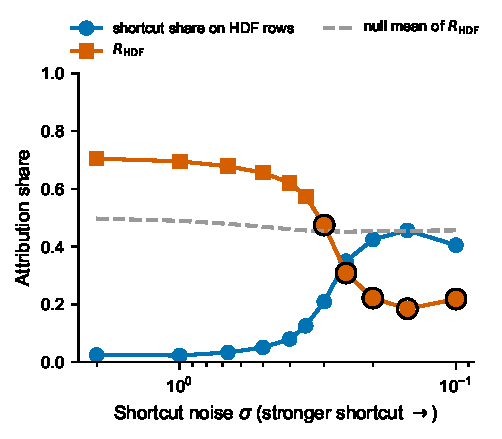
\includegraphics[width=0.52\textwidth]{shortcut_sweep.pdf}
\caption{Shortcut sweep. Circles mark noise levels at which the HDF relevant-share test fails.}
\label{fig:sweep}
\end{figure}

% Detection threshold
\Cref{tab:sweep,fig:sweep} show the shortcut sweep. For $\sigma \ge 0.5$ the sensor receives at most
4.4\% of the attribution on HDF rows and the audit passes, which is correct because the model barely
uses it. At $\sigma = 0.35$ the sensor takes 11\% and the audit still passes. From $\sigma = 0.25$,
where the sensor takes 36\%, the HDF relevant-share test fails, and from $\sigma = 0.15$ the
specificity test fails as well. Test F1 stays between 0.85 and 0.92 across the sweep, so accuracy
does not reveal the shortcut. H2 therefore holds for substantial reliance on a shortcut but not for
light reliance. PWF and OSF pass at every noise level. TWF fails its relevant-share test at the three
strongest shortcut levels, consistent with its weak result above.

\subsection{Resampling and feature-space structure}
\label{sec:structure}

\begin{figure}[htbp]
\centering
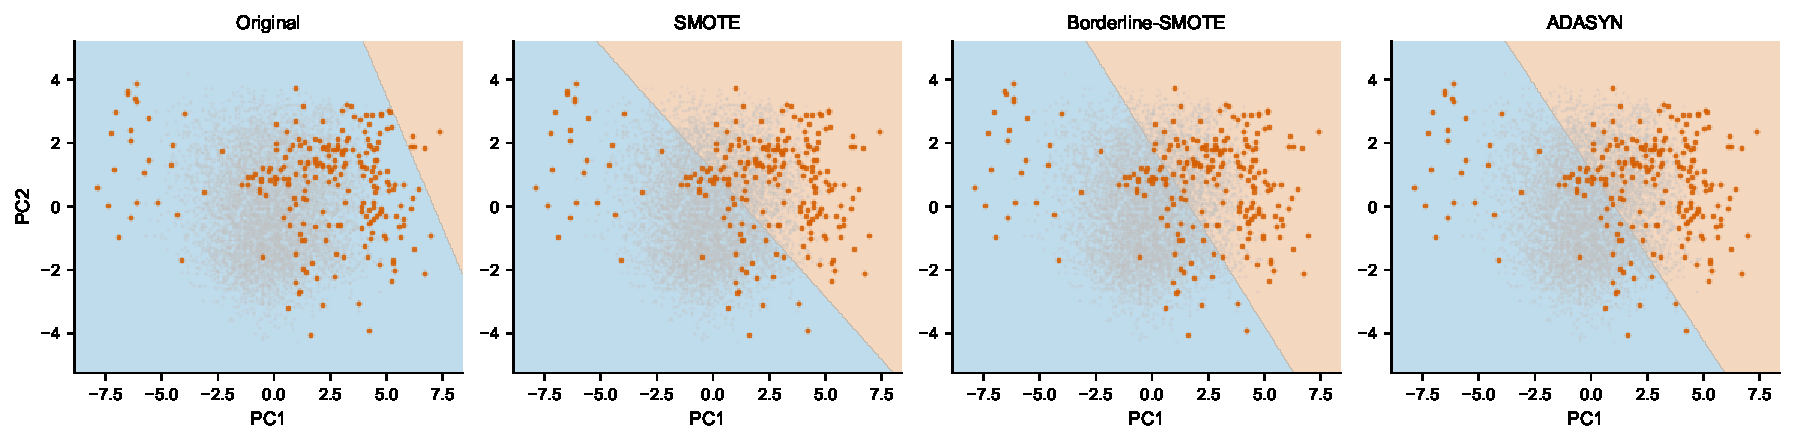
\includegraphics[width=0.9\textwidth]{decision_boundary_2d.pdf}
\caption{Logistic regression decision boundary on a two-dimensional principal component analysis
(PCA) projection of the training data, for each resampler.}
\label{fig:boundary}
\end{figure}

\begin{figure}[htbp]
\centering
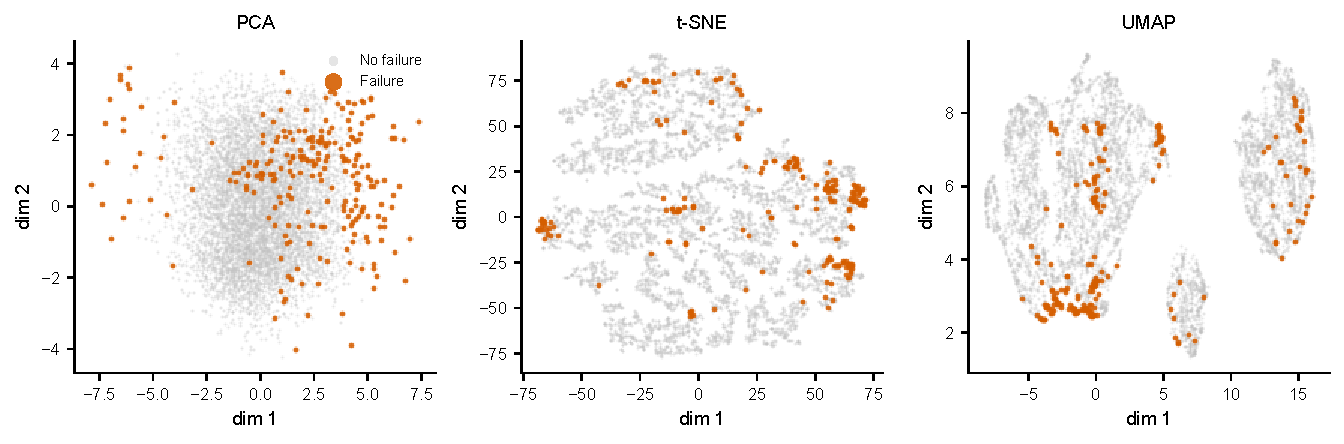
\includegraphics[width=0.78\textwidth]{dimred_comparison.pdf}
\caption{PCA, t-SNE, and UMAP projections of the training data, colored by \texttt{Machine failure}.}
\label{fig:dimred}
\end{figure}

\begin{table}[htbp]
\centering
\caption{Oversampler comparison on the validation set (default XGBoost).}
\label{tab:resamplers}
\footnotesize
\begin{tabular}{@{}lrrrr@{}}
\toprule
Sampler & Prec. & Rec. & F1 & PR-AUC \\
\midrule
Borderline-SMOTE & \textbf{0.814} & 0.838 & \textbf{0.826} & 0.883 \\
SMOTE & 0.699 & \textbf{0.853} & 0.768 & \textbf{0.892} \\
ADASYN & 0.683 & 0.824 & 0.747 & 0.876 \\
\bottomrule
\end{tabular}

\end{table}

% Resampling effect
Borderline-SMOTE has the highest validation F1 (\cref{tab:resamplers}). \Cref{fig:boundary} shows its
geometric effect on a logistic regression fitted to a two-dimensional PCA projection: without
resampling the decision boundary barely reaches the failure class, and each oversampler moves it
into the majority class, trading precision for recall.

% Structure consistent with several mechanisms
\Cref{fig:dimred} projects the training data with PCA, t-distributed stochastic neighbor embedding
(t-SNE)~\cite{vandermaaten2008tsne}, and uniform manifold approximation and projection
(UMAP)~\cite{mcinnes2018umap}. The classes overlap in the linear projection, consistent with the low
F1 of the linear models, while failures form several separate groups in the nonlinear ones,
consistent with several distinct mechanisms. The groups persist at t-SNE perplexities from 5 to
100 (repository figure), which matters because t-SNE shapes depend on
perplexity~\cite{wattenberg2016misread}.

\subsection{Limitations}
\label{sec:limits}

% Synthetic ground truth
AI4I~2020 is simulated from the same rules we use as ground truth, so the audit checks agreement
with the simulator's logic, not with independent measurements of real machines; we contribute a
protocol, not a finding about real equipment. Autran et al.~\cite{autran2024ai4ipmdi} show that
realistic irregularities added to AI4I~2020 change model performance, so results on the clean data
may not transfer.

% Audit-specific
The audit detects heavy reliance on a shortcut but not light reliance, it needs the trigger features
$E_m$ to be known, and the derived features influence its outcomes. We audit one model family with
one explainer on one dataset of 10{,}000 rows; mechanisms with few rows, such as TWF and RNF, give
weak evidence either way.

\section{Conclusion}
\label{sec:conclusion}

% Recap
We audited SHAP explanations of a PdM classifier against failure mechanisms that the model never
saw. With out-of-sample attributions, a model-randomization null, and Holm correction, the tuned
model's explanations match the heat dissipation, power, and overstrain mechanisms in all five seeds,
but not tool wear failure, which passes only when SHAP is computed on training rows. The audit flags
a shortcut sensor once it carries about a third of the attribution, while accuracy stays unchanged.
A naive null that compares random failure rows under the same model passes a permuted-label model,
so subgroup attribution tests need a null that accounts for how atypical the audited rows are.

% Future work
The audit applies wherever maintenance records log a root cause for failures that a model predicts
as a binary risk; we have not measured how common such records are. Next steps are real maintenance
logs with recorded root causes, other explainers and model families, and a formal power analysis of
the shortcut threshold.

\section*{Acknowledgment}
Portions of the manuscript text and the analysis code were drafted with the assistance of an AI
system (Claude, Anthropic). The author reviewed and verified all content and takes full
responsibility for it. Code, model artifacts, and scripts that regenerate every number, table, and
figure are available at \url{https://github.com/kowshik24/glowing-broccoli}.

\bibliographystyle{plainnat}
\bibliography{refs}

\end{document}
